% Chapter 2

\chapter{DSL Specification with CINCO}\label{ch:DSL}
This chapter explains the specification underlying the user documentation model. It is a textual DSL used to generate the graphical model element. The chapter starts by giving a overview of the framework in use and the boilerplate code coming with it. It then continues with the main aspects of the meta graph language and the meta style language as well as the cinco product definition. Finally, important key points of the Xtend generator classes are provided.
\section{CINCO SCCE Meta Tooling Framework}\label{sec:CTF}
The CINCO Framework is one of the many projects of the SCCE Group, which aims at allowing the application experts, rather than programming experts, to take charge of the development tasks~\cite{scce}. It is a generator-driven development environment for graphical domain-specific modeling tools. As for many software frameworks, the purpose to ease the development process by hiding the complexity of the underlying APIs and also by offering a selective integration of custom user-written code. Hence, it is reusable and application specific. The framework is based on the Eclipse Modeling Framework (EMF) and Graphiti Graphical Tooling Infrastructure~\cite{Cinco}. The widely spread Eclipse's Integrated Development Environment (IDE) provides the necessary support and a certain familiarity with the editor, which makes it easy to use for software development.
\begin{figure}[h]
    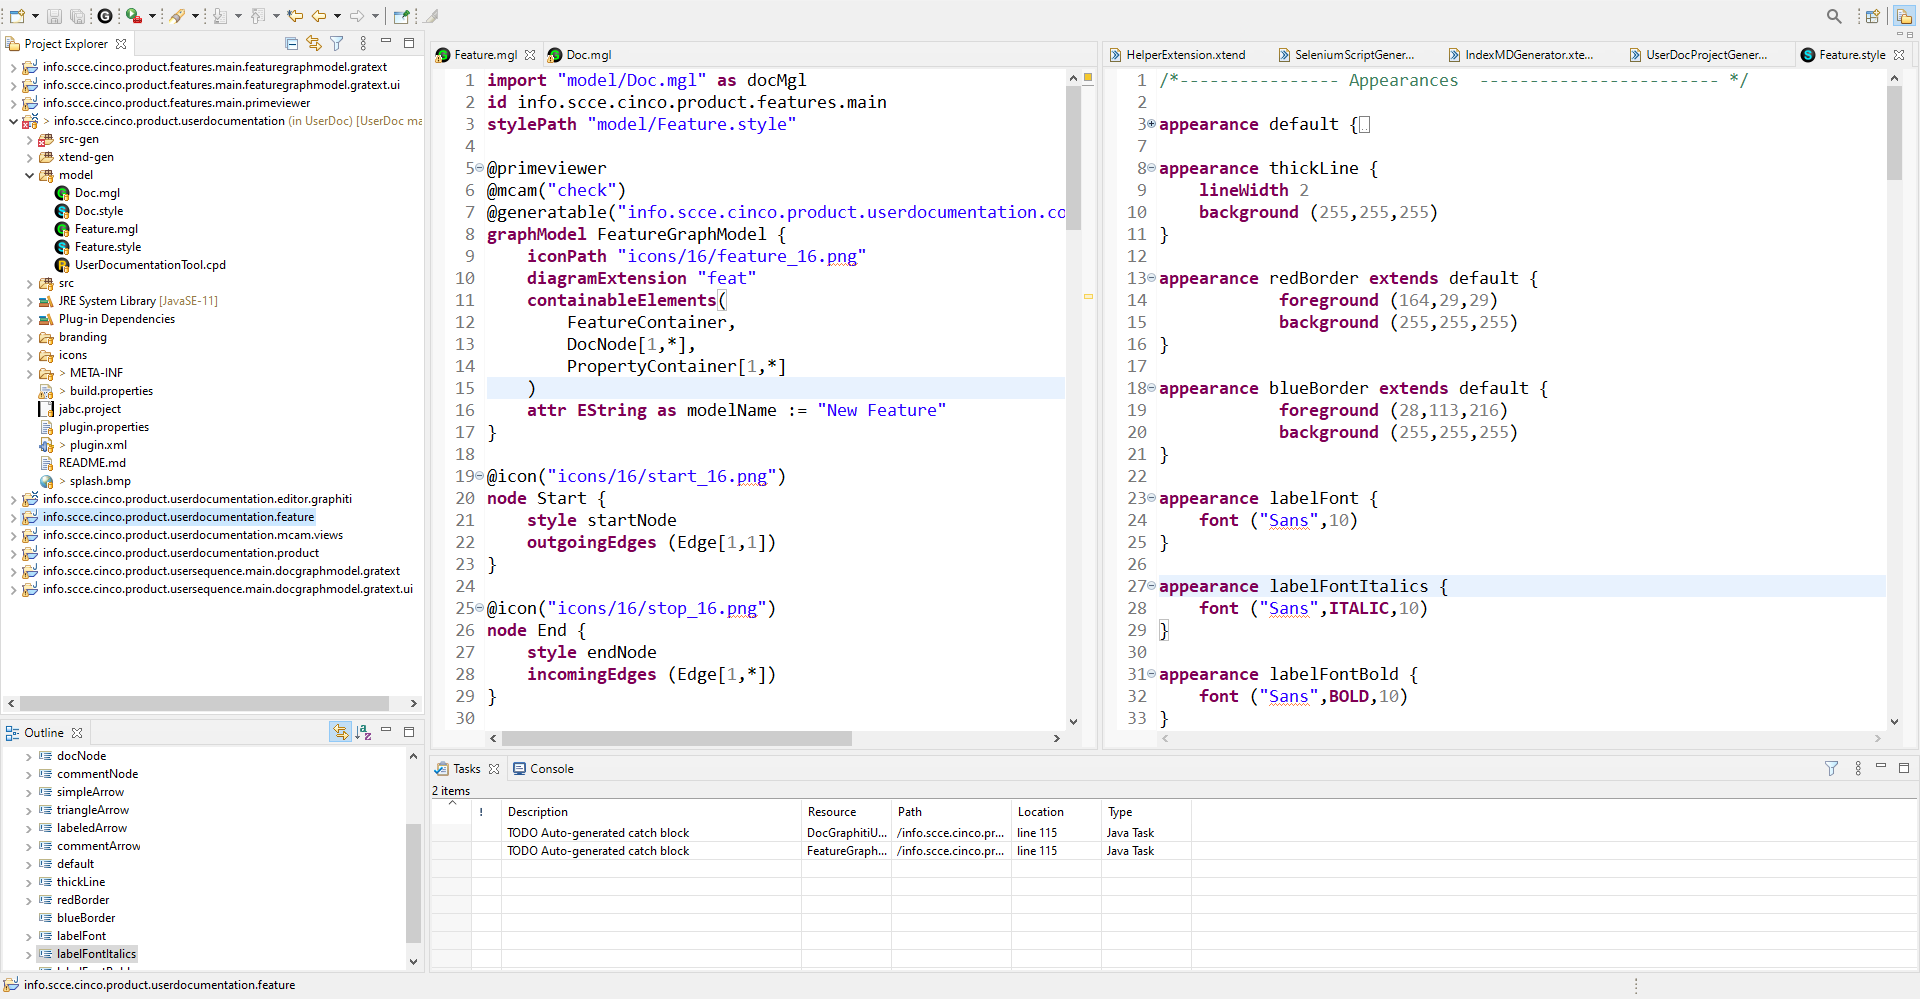
\includegraphics[width=\textwidth]{Cinco_EMF-Editor}
    \caption{The look of the CINCO IDE based on Eclipse}
\end{figure}

The term \textit{Meta} indicates that the tooling suite proposes a solution for the meta-specification of the corresponding domain-specific modeling tool. That means, the developer specifies the behavior and restrictions of the resulting graphical domain-specific modeling tool. Applying the concept of specialization at higher level brings much more control over the definition of the modeling tool and hence simplifies the development process. In this regard, the CINCO framework offers a push-button generation from the meta-specification~\cite{scce}. The generated editor instance is also an Eclipse-based editor, that can as well generate and execute programs on its turn, based on the tailored graphical model.

Xtext is used to define the textual syntax of the meta-specification that defines the appearance and structure of the model elements.

A specific Ecore metamodel for each tool is generated, with its corresponding editor based on Graphiti framework.


\section{Meta Graph Language}\label{sec:MGL}
\section{Meta Style Language}\label{sec:MSL}
\section{Cinco Product Definition}\label{sec:CPD}
\section{Xtend Generators}\label{sec:GEN}
